\documentclass[journal]{IEEEtran}

\ifCLASSINFOpdf

\else

\fi


\hyphenation{op-tical net-works semi-conduc-tor}
\usepackage{hyperref}
\usepackage{graphicx}
\usepackage{float}
\usepackage{caption}

\begin{document}



\title{Árbol de búsqueda binario autoequilibrado.\\(AVL tree)}



\author
    {Jose Pablo~Herrera Vargas, {Miembro del:~Tecnologíco de Costa Rica,}
        \\Esteban~Vargas Fernández, {Miembro del:~Tecnologíco de Costa Rica,}
        and~ \\Santiago Chavarria Azofeifa, {Miembro del:~Tecnologíco de Costa Rica.}

}

\markboth{Proyecto de investigación \LaTeX\ Octubre~2023}
{Shell \MakeLowercase{\textit{et al.}}: Bare Demo of IEEEtran.cls for IEEE Journals}

\maketitle


\begin{abstract}
Este documento científico se enfoca en la teoría de los árboles de búsqueda binaria autoequilibrados (AVL). Su lectura es esencial para comprender la diferencia entre los árboles AVL y los árboles de búsqueda binaria estándar (BST), así como para aprender a reconocer y abordar desequilibrios en un árbol AVL debido a inserciones o eliminaciones de nodos. Además, no te pierdas la oportunidad de adentrarte en el mundo de la optimización de datos. Descubre como las fascinantes aplicaciones que conciernen este tipo de estructuras de datos cambian y facilitan nuestra vida cotidiana.
\end{abstract}


\begin{IEEEkeywords}
 Árboles binarios , AVL, Binary Search Tree
\end{IEEEkeywords}

\IEEEpeerreviewmaketitle



\section{Introducción}

\IEEEPARstart{L}{a} 
presente investigación se centra en la teoría referente a los árboles de búsqueda binario autoequilibrados (AVL). Mediante la lectura de los contenidos establecidos se pretende que los estudiantes comprendan el concepto de árboles AVL y los distingan de los BST. Además, se espera que el estudiante reconozca los tipos de rotaciones que se deben aplicar en caso de algún desequilibrio dentro del árbol a causa de la inserción o eliminación de nodos.
 \cite{Experiencia en la construcción de Objetos de Aprendizaje}
 
\subsection{Datos históricos}
Los árboles AVL llevan su nombre en honor a los matemáticos G. M. Adelson-Velsky y E. M. Landis, quienes inventaron los métodos para construir estos árboles binarios en 1962. Fueron inventados para resolver el problema de los árboles de búsqueda binarios desequilibrados. Entre las operaciones que se realizan con este árbol incluyen: búsqueda, inserción y eliminación \cite{Section.io}, \cite{Estructuras de datos con C++ (2a. ed.)}

\subsection{Método de funcionamiento}

Árbol AVL es una variante especial de un Árbol de Búsqueda Binaria (BST) que se asegura de mantener un equilibrio adecuado en su estructura. Difiere de un BST, puesto que cada nodo del árbol tiene un factor de equilibrio. El factor de equilibrio de un nodo viene dado por el cálculo de la diferencia de alturas entre su subárbol izquierdo y subárbol derecho. Si el factor de equilibrio es -1, 0 o 1 se dice que el nodo esta equilibrado, pero con cualquier otro valor se considera que el nodo esta desequilibrado. En caso de existir un nodo desequilibrado entonces el árbol también lo estará y requerirá un reequilibrio \cite{AVL Trees with Relaxed Balance}. Para garantizar este equilibrio, se utilizan operaciones llamadas "rotaciones" cuando se detecta un desequilibrio en el árbol. Estas rotaciones reorganizan los nodos disminuyendo en el proceso la altura total del árbol en 1 unidad de esta forma el árbol se reequilibra y además, lo hace respetando las propiedades de un BST \cite{Data Structure and Algorithms}. Las rotaciones se realizan de cuatro formas diferentes dependiendo del caso en cuestión:
\\
Rotación II: Esta rotación se aplica cuando el factor de equilibrio de un nodo (en este caso C) se vuelve mayor que 1 debido a la inserción de un nodo en el subárbol izquierdo del subárbol izquierdo de C. A esta rotación, también se le conoce como rotación simple a la derecha porque se puede arreglar usando una sola operación de rotación hacia la derecha en el nodo desequilibrado. 

\begin{figure}[H]
    \centering
    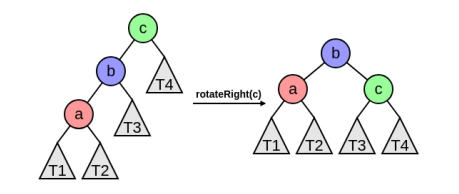
\includegraphics[scale=0.7]{LL rotation.PNG}
    \captionsetup{justification=centering}  % Alinea la leyenda al centro
    \caption{Rotación simple a la derecha \cite{Algoritmos y Programación}.}
    \label{fig:enter-label}

\end{figure}

Rotación DD: Esta rotación es inversa a la rotación LL, puesto que se aplica cuando el factor de equilibrio de un nodo (en este caso A) se vuelve menor que -1 debido a la inserción de un nodo en el subárbol derecho del subárbol derecho de A. También se le conoce como rotación simple a la izquierda porque se puede arreglar usando una sola operación de rotación hacia la izquierda en el nodo desequilibrado.

\begin{figure}[H]
    \centering
    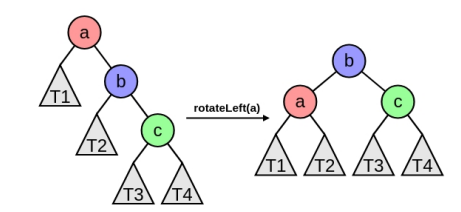
\includegraphics[scale=0.7]{RR rotation.PNG}
    \captionsetup{justification=centering}  % Alinea la leyenda al centro
    \caption{Rotación simple a la izquierda \cite{Algoritmos y Programación}.}
    \label{fig:enter-label}
\end{figure}

Rotación ID: Esta rotación se lleva a cabo cuando el factor de equilibrio de un nodo (en este caso C) se vuelve mayor que 1 debido a la inserción de un nodo en el subárbol derecho del subárbol izquierdo de C. También se puede ver como una operación compuesta que combina una rotación izquierda y una rotación derecha para restablecer el equilibrio del árbol.

\begin{figure}[H]
    \centering
    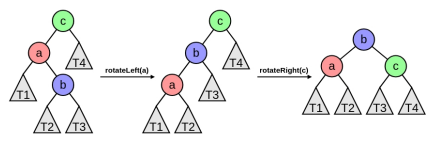
\includegraphics[scale=0.7]{LR rotation.PNG}
    \captionsetup{justification=centering}  % Alinea la leyenda al centro
    \caption{Rotación izquierda - derecha \cite{Algoritmos y Programación}.}
    \label{fig:enter-label}
\end{figure}

Rotación DI: Esta rotación se lleva a cabo cuando el factor de equilibrio de un nodo (en este caso A) se vuelve menor que -1 debido a la inserción de un nodo en el subárbol izquierdo del subárbol derecho de A. La rotación Derecha-Izquierda es una operación compuesta que combina una rotación derecha y una rotación izquierda para restablecer el equilibrio del árbol. 

\begin{figure}[H]
    \centering
    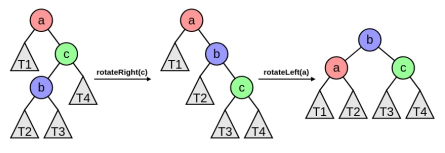
\includegraphics[scale=0.7]{RL rotation.PNG}
    \captionsetup{justification=centering}  % Alinea la leyenda al centro
    \caption{Rotación derecha - izquierda \cite{Algoritmos y Programación}.}
    \label{fig:enter-label}
\end{figure}

\subsection{Método de utilización}

Los métodos utilizados en este tipo de árbol, al igual que en el BST, son la inserción y la eliminación. La parte de la codificación en la inserción utiliza la misma lógica que en el inicio: mayores a la derecha y menores a la izquierda. La diferencia radica en que, después de la inserción, se evalúa y compara la altura del árbol desde el nodo recién incluido hasta la raíz principal del árbol, y, en caso necesario, se realizan rotaciones. Lo mismo ocurre en el caso de la eliminación, donde se utilizan los mismos métodos que en un BST convencional, además de la evaluación y comparación de alturas de cada subárbol para llevar a cabo las rotaciones necesarias.

Gracias a esta disposición, funciones como máximo o mínimo requieren menos ciclos para obtener un resultado, de igual manera, según \cite{AVL Aplications}, el árbol AVL se utiliza recientemente en muchas aplicaciones; se utiliza en entornos de cómputo en la nube para la programación de tareas. \cite{web index} Propone un algoritmo para indexar las palabras clave extraídas de documentos web junto con su contexto, basado en un árbol AVL. Se ha utilizado en redes de sensores inalámbricos para proporcionar un protocolo de seguridad. Además, se ha implementado esta estructura en la clasificación de minería de datos para la inducción de un árbol de decisiones.

\section{Demostración}
Para ejemplificar como se ve y funcionan los arboles AVL,
se da la opción de usar esta pagina de visualización de los mismos: \cite{Demostracion}

\section{Conclusión y Recomendaciones}
Se determina que la disposición y eficiencia de los árboles AVL tiene un impacto significativo en diversas aplicaciones de la vida, son una opción poderosa para mantener árboles binarios de búsqueda equilibrados, pero tienen ciertas limitaciones en términos de consumo de recursos y complejidad de implementación. Su elección debe basarse en los requisitos específicos de su aplicación y en las operaciones que realiza con mayor frecuencia.\\

En caso de necesitar material adicional para una mejor comprención del tema se recomienda observar el siguiente video que resume los contenidos desarrollados: \cite{video}

%%%%%%%%%%%%%%%%%%%%%%%%%%%%%%%%%%%%%%%%%%%%%%%%%%%%%%%%%%%%%%%%%%%

\begin{thebibliography}{10}

\bibitem{Experiencia en la construcción de Objetos de Aprendizaje}
Catalina Mostaccio, Gabriela Pérez. \textit{Experiencia en la construcción de Objetos de Aprendizaje para árboles AVL usando CROA}, LIFIA – Facultad de Informática de la Universidad Nacional de La Plata, 2015. 
[Consultado 15-oct-2023]

\bibitem{Section.io}
"Introduction to AVL trees", \textit{Section}, Disponible en:
\url{https://www.section.io/engineering-education/introduction-to-avl-trees/} [En linea] 
[Consultado 14-oct-2023]

\bibitem{Estructuras de datos con C++ (2a. ed.)} 
Malik Davender S, \textit{Estructuras de datos con C++ (2a. ed.)}, Cengage Learning, 2013. 
[Consultado 14-oct-2023]


\bibitem {AVL Trees with Relaxed Balance} Kim S. Larsen .\textit{AVL Trees with Relaxed Balance} University of Southern Denmark, 2000. 
[Consultado 16-oct-2023]

\bibitem{Data Structure and Algorithms} TutorialsPoint. \textit{Data Structure and Algorithms} [En línea], 2023.
[Consultado 16-oct-2023]

\bibitem{Algoritmos y Programación}
M. Méndez, \textit{Algoritmos y Programación II Tdá Arbol.}, Facultad De Ingeniería, Universidad de Buenos Aires, 2020.
[Consultado 16-oct-2023]

\bibitem{AVL Aplications} Bounif, Lynda, Djamel Eddine, Zegour. \textit{AVL and Red-black trees as a single balanced tree} 2016.
[Consultado 16-oct-2023]

\bibitem{web index} Tyagi, Nidhi, Rahul Rishi, and R. P. Aggarwal .\textit{Context based Web Indexing for Storage of Relevant Web Pages} International Journal of Computer Applications Vol40, 2012.
[Consultado 16-oct-2023]

\bibitem{Demostracion}
Demostración, Disponible en: \url{https://cs221viz.netlify.app/src/avl}, [En linea]

\bibitem{video}
Algoritmos Fiuba Curso Buchwald, Disponible en: 
\url{https://www.youtube.com/watch?v=PMcQvSM1OAM}, [En linea] 

\end{thebibliography}

\end{document}


